% ============================================================
%  Algebraic Reasoning Distiller  —  Flux Beamer  v3
%  Light background, dark banners, small fonts, generous spacing
% ============================================================
\documentclass[aspectratio=169,10pt]{beamer}

\usepackage[utf8]{inputenc}
\usepackage[T1]{fontenc}
\usepackage{amsmath,amssymb,amsfonts}
\usepackage{graphicx}
\usepackage{booktabs}
\usepackage{colortbl}
\usepackage{array}
\usepackage{xcolor}
\usepackage{tikz}
\usetikzlibrary{positioning,arrows.meta,fit,backgrounds,calc}

% ── Palette ─────────────────────────────────────────────────
\definecolor{SlideBackground}{HTML}{F4F6FB}   % almost-white
\definecolor{BannerDark}{HTML}{0D1117}         % near-black
\definecolor{BannerMid}{HTML}{1C2333}
\definecolor{AccentBlue}{HTML}{1E6FBF}
\definecolor{AccentCyan}{HTML}{0892C8}
\definecolor{AccentGreen}{HTML}{1A8C58}
\definecolor{AccentRed}{HTML}{C0392B}
\definecolor{AccentGold}{HTML}{B07D10}
\definecolor{AccentPurple}{HTML}{6A3E9E}
\definecolor{TextDark}{HTML}{1A1A2A}
\definecolor{TextMid}{HTML}{3A3A4A}
\definecolor{TextLight}{HTML}{F0F4FF}
\definecolor{BoxBg}{HTML}{E8EDF8}
\definecolor{BoxBgAlt}{HTML}{EAF5EA}

% ── Beamer colours ──────────────────────────────────────────
\setbeamercolor{background canvas}{bg=SlideBackground}
\setbeamercolor{normal text}{fg=TextDark}
\setbeamercolor{footline}{bg=BannerMid, fg=TextLight}
\setbeamercolor{frametitle}{fg=TextLight, bg=BannerDark}
\setbeamercolor{framesubtitle}{fg=AccentCyan}
\setbeamercolor{title}{fg=TextLight}
\setbeamercolor{structure}{fg=AccentBlue}
\setbeamercolor{itemize item}{fg=AccentBlue}
\setbeamercolor{itemize subitem}{fg=AccentCyan}
\setbeamercolor{block title}{bg=AccentBlue, fg=white}
\setbeamercolor{block body}{bg=BoxBg, fg=TextDark}
\setbeamercolor{alerted text}{fg=AccentRed}

% ── Fonts & sizes ───────────────────────────────────────────
\setbeamerfont{frametitle}{size=\small, series=\bfseries}
\setbeamerfont{framesubtitle}{size=\footnotesize}
\setbeamerfont{normal text}{size=\footnotesize}
\setbeamerfont{itemize/enumerate body}{size=\footnotesize}
\setbeamerfont{block title}{size=\footnotesize, series=\bfseries}
\setbeamerfont{block body}{size=\scriptsize}

% ── Templates ───────────────────────────────────────────────
\setbeamertemplate{navigation symbols}{}
\setbeamertemplate{itemize item}{\scriptsize$\blacktriangleright$}
\setbeamertemplate{itemize subitem}{\scriptsize$\triangleright$}

\setbeamertemplate{frametitle}{%
  \vskip0pt
  \begin{beamercolorbox}[wd=\paperwidth,ht=8mm,dp=2mm,leftskip=5mm]{frametitle}%
    \vbox to 8mm{\vfil
      \hbox{\usebeamerfont{frametitle}\insertframetitle
      \ifx\insertframesubtitle\@empty\else
        \hspace{3mm}\textcolor{AccentCyan}{\normalfont\footnotesize|}\hspace{3mm}%
        \textcolor{AccentCyan}{\usebeamerfont{framesubtitle}\insertframesubtitle}%
      \fi}%
    \vfil}%
  \end{beamercolorbox}%
}

\setbeamertemplate{footline}{%
  \begin{beamercolorbox}[wd=\paperwidth,ht=5mm,dp=1.5mm]{footline}%
    \vbox to 5mm{\vfil
      \hbox to \paperwidth{%
        \hspace{4mm}%
        \textcolor{TextLight}{\tiny Algebraic Reasoning Distiller}%
        \hfill
        \textcolor{TextLight}{\tiny SAIR — Mathematics Distillation Challenge}%
        \hfill
        \textcolor{AccentCyan}{\tiny\insertframenumber/\inserttotalframenumber}%
        \hspace{4mm}}%
    \vfil}%
  \end{beamercolorbox}%
}

% ── Helpers ─────────────────────────────────────────────────
\newcommand{\hl}[1]{\textcolor{AccentRed}{\textbf{#1}}}
\newcommand{\cy}[1]{\textcolor{AccentBlue}{\textbf{#1}}}
\newcommand{\gn}[1]{\textcolor{AccentGreen}{\textbf{#1}}}
\newcommand{\gd}[1]{\textcolor{AccentGold}{\textbf{#1}}}

% content area margin helper
\newcommand{\slidepad}{\vspace{3mm}\hspace{2mm}}

% ── TikZ node styles ────────────────────────────────────────
\tikzset{
  ND/.style={draw=#1, fill=#1!10, rounded corners=3pt,
             inner sep=5pt, align=center, text=TextDark, font=\scriptsize},
  ARR/.style={-Stealth, thick, #1},
}

% ============================================================
\begin{document}
\fontsize{9.5pt}{11.5pt}\selectfont
\footnotesize   % global default

% ============================================================
% SLIDE 1  ·  TITLE
% ============================================================
{
\setbeamertemplate{footline}{}
\begin{frame}[plain]

\begin{tikzpicture}[remember picture,overlay]
  % Full dark background
  \fill[BannerDark] (current page.north west) rectangle (current page.south east);
  % Cyan accent strip left
  \fill[AccentBlue] (current page.north west) rectangle
    ([xshift=8mm]current page.south west);
  % Top gradient panel
  \fill[BannerMid] (current page.north west) rectangle
    ([yshift=-45mm]current page.north east);
  % Decorative triangles
  \begin{scope}[opacity=0.06]
    \fill[AccentCyan]
      ([xshift=0.55\paperwidth]current page.north west) --
      ([xshift=\paperwidth]current page.north west) --
      ([xshift=\paperwidth,yshift=-45mm]current page.north west) -- cycle;
  \end{scope}
  % ACTIVE badge
  \node[fill=AccentRed, text=white, font=\bfseries\scriptsize,
        rounded corners=2pt, inner sep=4pt,
        anchor=north east, xshift=-6mm, yshift=-5mm]
    at (current page.north east) {ACTIVE  —  Deadline Apr 20, 2026};
  % Main title
  \node[anchor=west, xshift=14mm, yshift=14mm] at (current page.west){%
    \parbox{0.66\paperwidth}{%
      \textcolor{white}{\large\bfseries Algebraic Reasoning Distiller}\\[5pt]
      \textcolor{AccentCyan}{\normalsize
        Harnessing Multi-Agent Collaboration\\
        for Mathematical Problem Solving}\\[8pt]
      \textcolor{gray}{\scriptsize
        SAIR Foundation — Mathematics Distillation Challenge, Stage 1: Equational Theories}
    }};
  % Authors
  \node[anchor=south west, xshift=14mm, yshift=12mm]
    at (current page.south west){%
    \parbox{0.85\paperwidth}{%
      \textcolor{white}{\scriptsize
        Joaquín Mir Macías $\cdot$
        José Andrés Ridruejo Tuñón $\cdot$
        Javier Ríos Montes $\cdot$
        Miguel Montes Lorenzo}\\[2pt]
      \textcolor{gray}{\tiny
        Deep Generative Models $\cdot$ Master in Artificial Intelligence $\cdot$
        UPM 2025/2026}}};
\end{tikzpicture}
\end{frame}
}

% ============================================================
% SLIDE 2  ·  MOTIVATION
% ============================================================
\begin{frame}{Motivation}{Why does mathematical reasoning still fail?}
\begin{columns}[T,onlytextwidth]
  \begin{column}{0.50\textwidth}
    \vspace{2mm}
    \cy{The gap in LLM mathematical reasoning:}
    \vspace{1mm}
    \begin{itemize}\setlength\itemsep{2pt}
      \item LLMs solve math by \hl{pattern matching}, not symbolic understanding
      \item Consistent errors in algebraic manipulation and abstract inference
      \item \textbf{Pretraining} on math corpora is prohibitively expensive
      \item Naive \textbf{fine-tuning} produces narrow experts
      \item Even frontier models show weaknesses in abstract algebra
    \end{itemize}
    \vspace{2mm}
    \begin{block}{Our approach}
      \textbf{Symbolic reasoning} + \textbf{LLM distillation} via
      multi-agent offline computation, within strict competition constraints.
    \end{block}
  \end{column}
  \hfill
  \begin{column}{0.44\textwidth}
    \vspace{4mm}
    % IMAGE PLACEHOLDER
    % Suggested: bar chart (matplotlib, light bg) comparing accuracy on
    % algebraic benchmarks: Base model vs. SFT vs. ARD.
    % Colors: AccentBlue / AccentGreen / AccentRed bars.
    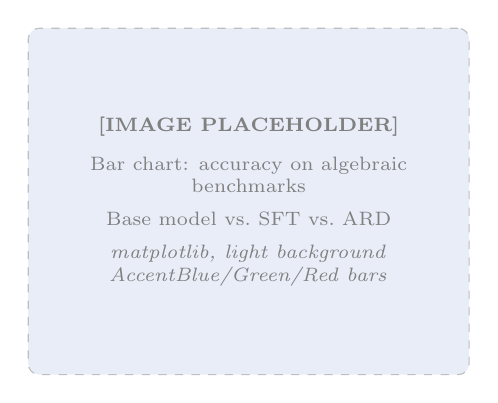
\begin{tikzpicture}
      \node[draw=gray!50, dashed, fill=BoxBg,
            rounded corners=4pt, minimum width=5.6cm, minimum height=4.4cm,
            align=center, text=gray, font=\scriptsize]{%
        \textbf{[IMAGE PLACEHOLDER]}\\[6pt]
        Bar chart: accuracy on algebraic\\
        benchmarks\\[4pt]
        Base model vs.\ SFT vs.\ ARD\\[4pt]
        \textit{matplotlib, light background}\\
        \textit{AccentBlue/Green/Red bars}
      };
    \end{tikzpicture}
  \end{column}
\end{columns}
\end{frame}

% ============================================================
% SLIDE 3  ·  PROBLEM STATEMENT
% ============================================================
\begin{frame}{The Challenge}{SAIR — Mathematics Distillation Challenge}
\begin{columns}[T,onlytextwidth]
  \begin{column}{0.50\textwidth}
    \vspace{4mm}
    \cy{Mathematical formulation:}
    \vspace{3mm}

    A \textbf{magma} is a set $M$ with a binary operation
    ${\ast}:M\!\times\!M\to M$ \textit{(no axioms assumed)}.

    \vspace{4mm}
    Given $E_1, E_2$ built with $\ast$, decide:
    \[
      \boxed{\;E_1 \;\overset{?}{\Longrightarrow}\; E_2
             \;\text{ in every magma}\;}
    \]

    \vspace{4mm}
    \textbf{Example:}\\[3pt]
    $E_1{:}\; x \ast y = z \ast (w \ast (u \ast u))$\\[2pt]
    $E_2{:}\; x \ast (y \ast y) = (z \ast w) \ast z$\\[4pt]
    \gn{Answer: TRUE}
    \hfill\textcolor{gray}{\tiny every magma satisfying $E_1$ also satisfies $E_2$}
  \end{column}
  \hfill
  \begin{column}{0.46\textwidth}
    \vspace{2mm}
    \cy{Competition constraints:}
    \vspace{2mm}

    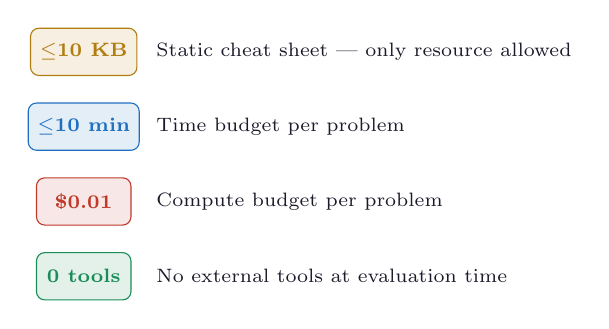
\begin{tikzpicture}[every node/.style={font=\scriptsize}]
      \foreach \y/\col/\badge/\desc in {
        0.0/AccentGold/{$\leq$10 KB}/{Static cheat sheet — only resource allowed},
        -0.95/AccentBlue/{$\leq$10 min}/{Time budget per problem},
        -1.90/AccentRed/{\$0.01}/{Compute budget per problem},
        -2.85/AccentGreen/{0 tools}/{No external tools at evaluation time}
      }{
        \node[draw=\col, fill=\col!12, rounded corners=3pt,
              minimum width=1.2cm, minimum height=6mm,
              font=\bfseries\scriptsize, text=\col, align=center]
          at (0,\y) {\badge};
        \node[anchor=west, text=TextDark] at (0.8,\y) {\desc};
      }
    \end{tikzpicture}

    \vspace{4mm}
    \begin{block}{Key insight}
      All heavy compute happens \textbf{offline}.
      At test time: cheat sheet + one LLM call.
    \end{block}
  \end{column}
\end{columns}
\end{frame}

% ============================================================
% SLIDE 4  ·  SYSTEM ARCHITECTURE
% ============================================================
\begin{frame}{System Architecture}{ARD — Algebraic Reasoning Distiller}
\vspace{1mm}
\centering
\resizebox{0.96\textwidth}{!}{%
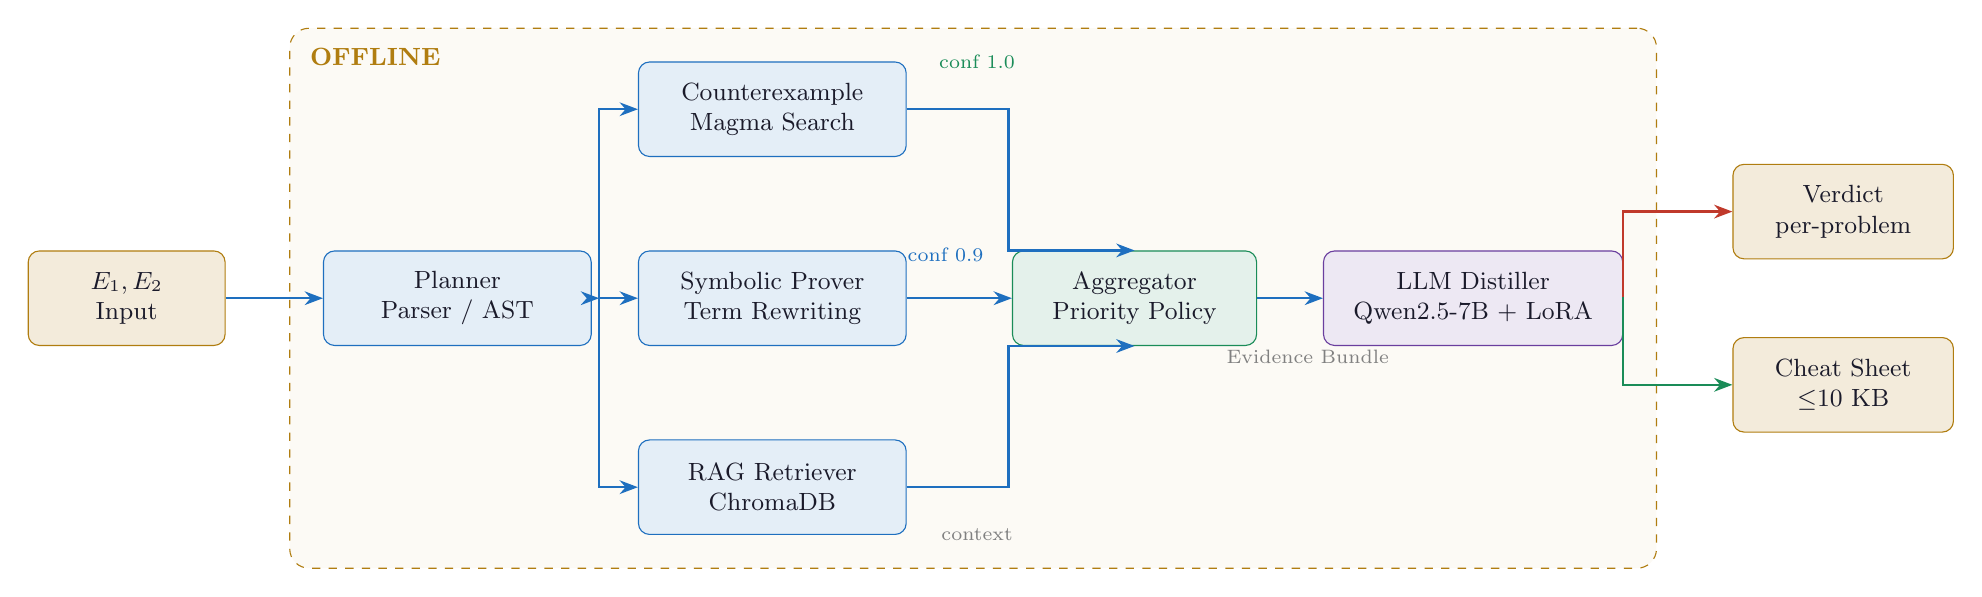
\begin{tikzpicture}[
  every node/.style={font=\small},
  IN/.style={draw=AccentGold,   fill=AccentGold!15,   rounded corners=4pt,
             minimum height=12mm, minimum width=25mm,
             align=center, text=TextDark},
  OT/.style={draw=AccentGold,   fill=AccentGold!15,   rounded corners=4pt,
             minimum height=12mm, minimum width=28mm,
             align=center, text=TextDark},
  AG/.style={draw=AccentBlue,   fill=AccentBlue!12,   rounded corners=4pt,
             minimum height=12mm, minimum width=34mm,
             align=center, text=TextDark},
  GR/.style={draw=AccentGreen,  fill=AccentGreen!12,  rounded corners=4pt,
             minimum height=12mm, minimum width=31mm,
             align=center, text=TextDark},
  LM/.style={draw=AccentPurple, fill=AccentPurple!12, rounded corners=4pt,
             minimum height=12mm, minimum width=38mm,
             align=center, text=TextDark},
  arr/.style={-Stealth, thick, AccentBlue},
  darr/.style={-Stealth, thick, AccentRed},
  garr/.style={-Stealth, thick, AccentGreen},
]

  % Main nodes
  \node[IN] (inp)  at (-1.0, 0.0) {$E_1,E_2$\\Input};
  \node[AG] (plan) at (3.2, 0.0) {Planner\\Parser / AST};

  \node[AG] (cex)  at (7.2, 2.4) {Counterexample\\Magma Search};
  \node[AG] (sym)  at (7.2, 0.0) {Symbolic Prover\\Term Rewriting};
  \node[AG] (rag)  at (7.2,-2.4) {RAG Retriever\\ChromaDB};

  \node[GR] (agg)  at (11.8, 0.0) {Aggregator\\Priority Policy};
  \node[LM] (llm)  at (16.1, 0.0) {LLM Distiller\\Qwen2.5-7B + LoRA};

  \node[OT] (verd) at (20.8, 1.1) {Verdict\\per-problem};
  \node[OT] (cs)   at (20.8,-1.1) {Cheat Sheet\\$\leq$10 KB};

  % Branch helper coordinates
  \coordinate (fork1) at (5.0, 0.0);
  \coordinate (joinTop) at (10.2, 2.4);
  \coordinate (joinBot) at (10.2,-2.4);
  \coordinate (outSplit) at (18.0, 0.0);

  % Arrows
  \draw[arr] (inp.east) -- (plan.west);
  \draw[arr] (plan.east) -- (fork1);
  \draw[arr] (fork1) |- (cex.west);
  \draw[arr] (fork1) -- (sym.west);
  \draw[arr] (fork1) |- (rag.west);

  \draw[arr] (cex.east) -- (joinTop) |- (agg.north);
  \draw[arr] (sym.east) -- (agg.west);
  \draw[arr] (rag.east) -- (joinBot) |- (agg.south);

  \draw[arr] (agg.east) -- (llm.west);
  \draw[darr] (llm.east) -- (outSplit) |- (verd.west);
  \draw[garr] (llm.east) -- (outSplit) |- (cs.west);

  % Labels
  \node[font=\scriptsize, text=AccentGreen] at (9.8, 3.0) {conf 1.0};
  \node[font=\scriptsize, text=AccentBlue]  at (9.4, 0.55) {conf 0.9};
  \node[font=\scriptsize, text=gray]        at (9.8,-3.0) {context};
  \node[font=\scriptsize, text=gray]        at (14.0,-0.75) {Evidence Bundle};

  % Offline box
  \begin{scope}[on background layer]
    \node[draw=AccentGold, dashed, fill=AccentGold!4,
          rounded corners=7pt,
          fit=(plan)(cex)(sym)(rag)(agg)(llm),
          inner sep=12pt] (offbox) {};
  \end{scope}

  \node[font=\small\bfseries, text=AccentGold,
        anchor=north west, xshift=4pt, yshift=-4pt]
    at (offbox.north west) {OFFLINE};

\end{tikzpicture}%
}
\end{frame}

% ============================================================
% SLIDE 5  ·  PLANNER
% ============================================================
\begin{frame}{Agent: Planner}{Parsing equations into Abstract Syntax Trees}
\begin{columns}[T,onlytextwidth]
  \begin{column}{0.46\textwidth}
    \vspace{4mm}
    \cy{Recursive-descent parser}\\[5pt]
    Input string $\to$ nested tuple AST:

    \vspace{6mm}
    \centering
    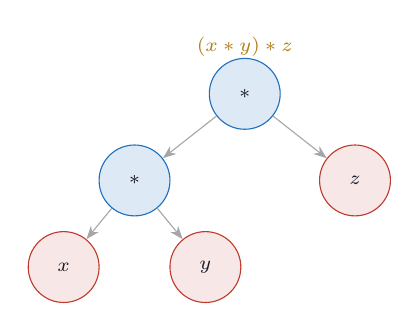
\begin{tikzpicture}[
      nd/.style={circle, draw=AccentBlue, fill=AccentBlue!15,
                 text=TextDark, font=\scriptsize,
                 inner sep=0pt, minimum size=9mm},
      lf/.style={circle, draw=AccentRed, fill=AccentRed!12,
                 text=TextDark, font=\scriptsize,
                 inner sep=0pt, minimum size=9mm},
      ar/.style={-Stealth, gray!70, thin},
    ]
      \node[font=\scriptsize, text=AccentGold] at (0, 0.6) {$(x \ast y)\ast z$};
      \node[nd] (r)  at (0,  0)   {$\ast$};
      \node[nd] (l)  at (-1.4,-1.1) {$\ast$};
      \node[lf] (rr) at ( 1.4,-1.1) {$z$};
      \node[lf] (ll) at (-2.3,-2.2) {$x$};
      \node[lf] (lr) at (-0.5,-2.2) {$y$};
      \draw[ar] (r)--(l); \draw[ar] (r)--(rr);
      \draw[ar] (l)--(ll); \draw[ar] (l)--(lr);
    \end{tikzpicture}

    \vspace{4mm}
    \centering\texttt{\scriptsize ("op", ("op","x","y"), "z")}
  \end{column}
  \hfill
  \begin{column}{0.50\textwidth}
    \vspace{4mm}
    \cy{Why ASTs?}
    \vspace{3mm}
    \begin{itemize}\setlength\itemsep{6pt}
      \item Canonical representation \textbf{shared by all agents}
      \item Enables structural comparison:\\
            alpha-equivalence, substitution
      \item Decouples \textbf{surface syntax} from mathematical content
      \item Variables: \texttt{("var","x")}\\
            Operations: \texttt{("op", left, right)}
    \end{itemize}
    \vspace{6mm}
    \begin{block}{Design principle}
      Every agent receives the same AST —
      errors propagate cleanly and the pipeline
      \textbf{never crashes} on malformed input.
    \end{block}
  \end{column}
\end{columns}
\end{frame}

% ============================================================
% SLIDE 6  ·  COUNTEREXAMPLE + SYMBOLIC
% ============================================================
\begin{frame}{Agents: Counterexample \& Symbolic Prover}{Hard evidence collection}
\begin{columns}[T,onlytextwidth]
  \begin{column}{0.48\textwidth}
    \vspace{4mm}
    \cy{Counterexample Generator}\\[4pt]
    \scriptsize Find magma $M$: $E_1$ holds, $E_2$ fails.

    \vspace{5mm}
    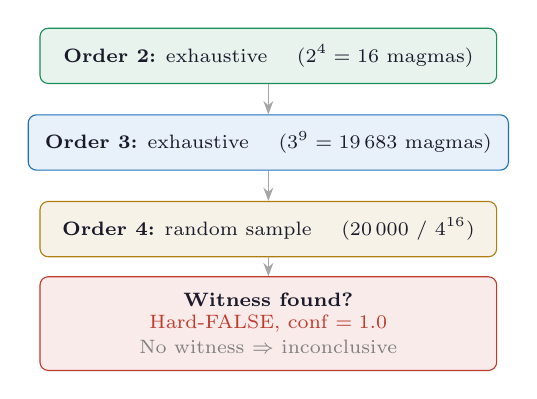
\begin{tikzpicture}[every node/.style={font=\scriptsize},
                        ar/.style={-Stealth,gray!70,thin}]
      \node[draw=AccentGreen, fill=AccentGreen!10, rounded corners=3pt,
            minimum width=5.8cm, inner sep=6pt, align=left, text=TextDark]
        (o2) at (0,0)
        {\textbf{Order 2:} exhaustive \quad ($2^4=16$ magmas)};
      \node[draw=AccentBlue, fill=AccentBlue!10, rounded corners=3pt,
            minimum width=5.8cm, inner sep=6pt, align=left, text=TextDark]
        (o3) at (0,-1.1)
        {\textbf{Order 3:} exhaustive \quad ($3^9=19\,683$ magmas)};
      \node[draw=AccentGold, fill=AccentGold!10, rounded corners=3pt,
            minimum width=5.8cm, inner sep=6pt, align=left, text=TextDark]
        (o4) at (0,-2.2)
        {\textbf{Order 4:} random sample \quad (20\,000 / $4^{16}$)};
      \node[draw=AccentRed, fill=AccentRed!10, rounded corners=3pt,
            minimum width=5.8cm, inner sep=6pt, align=center, text=TextDark]
        (res) at (0,-3.4)
        {\textbf{Witness found?}\\
         \textcolor{AccentRed}{Hard-FALSE, conf $= 1.0$}\\[1pt]
         \textcolor{gray}{No witness $\Rightarrow$ inconclusive}};
      \draw[ar](o2)--(o3); \draw[ar](o3)--(o4); \draw[ar](o4)--(res);
    \end{tikzpicture}
  \end{column}
  \hfill
  \begin{column}{0.48\textwidth}
    \vspace{4mm}
    \cy{Symbolic Prover}\\[4pt]
    \scriptsize Three strategies, applied in order:

    \vspace{5mm}
    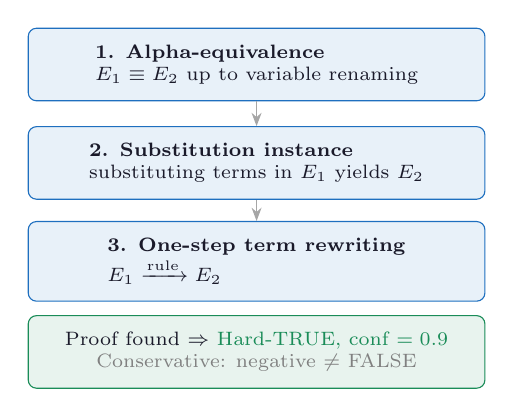
\begin{tikzpicture}[every node/.style={font=\scriptsize},
                        ar/.style={-Stealth,gray!70,thin}]
      \node[draw=AccentBlue, fill=AccentBlue!10, rounded corners=3pt,
            minimum width=5.8cm, inner sep=6pt, align=left, text=TextDark]
        (a1) at (0,0)
        {\textbf{1. Alpha-equivalence}\\
         $E_1 \equiv E_2$ up to variable renaming};
      \node[draw=AccentBlue, fill=AccentBlue!10, rounded corners=3pt,
            minimum width=5.8cm, inner sep=6pt, align=left, text=TextDark]
        (a2) at (0,-1.25)
        {\textbf{2. Substitution instance}\\
         substituting terms in $E_1$ yields $E_2$};
      \node[draw=AccentBlue, fill=AccentBlue!10, rounded corners=3pt,
            minimum width=5.8cm, inner sep=6pt, align=left, text=TextDark]
        (a3) at (0,-2.5)
        {\textbf{3. One-step term rewriting}\\
         $E_1 \xrightarrow{\text{rule}} E_2$};
      \node[draw=AccentGreen, fill=AccentGreen!10, rounded corners=3pt,
            minimum width=5.8cm, inner sep=6pt, align=center, text=TextDark]
        at (0,-3.65)
        {Proof found $\Rightarrow$
         \textcolor{AccentGreen}{Hard-TRUE, conf $= 0.9$}\\
         \textcolor{gray}{Conservative: negative $\neq$ FALSE}};
      \draw[ar](a1)--(a2); \draw[ar](a2)--(a3);
    \end{tikzpicture}
  \end{column}
\end{columns}
\end{frame}

% ============================================================
% SLIDE 7  ·  RAG + AGGREGATOR
% ============================================================
\begin{frame}{Agents: RAG Retriever \& Aggregator}{Context injection and priority policy}
\begin{columns}[T,onlytextwidth]
  \begin{column}{0.44\textwidth}
    \vspace{4mm}
    \cy{RAG Retriever}
    \vspace{5mm}

    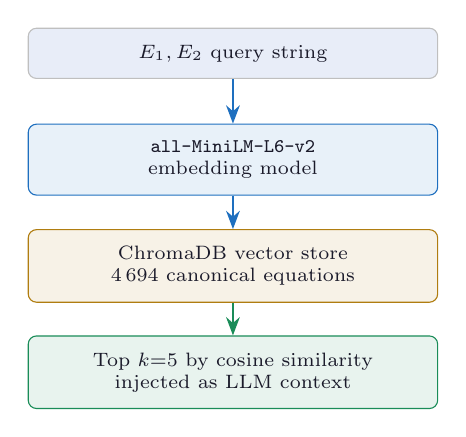
\begin{tikzpicture}[every node/.style={font=\scriptsize},
                        ar/.style={-Stealth,thick,AccentBlue}]
      \node[draw=gray!50,    fill=BoxBg,           rounded corners=3pt,
            minimum width=5.2cm, inner sep=6pt, align=center, text=TextDark]
        (q)  at (0, 0.0)   {$E_1, E_2$ query string};
      \node[draw=AccentBlue, fill=AccentBlue!10,  rounded corners=3pt,
            minimum width=5.2cm, inner sep=6pt, align=center, text=TextDark]
        (em) at (0,-1.35) {\texttt{all-MiniLM-L6-v2}\\embedding model};
      \node[draw=AccentGold, fill=AccentGold!10,  rounded corners=3pt,
            minimum width=5.2cm, inner sep=6pt, align=center, text=TextDark]
        (db) at (0,-2.70) {ChromaDB vector store\\4\,694 canonical equations};
      \node[draw=AccentGreen,fill=AccentGreen!10, rounded corners=3pt,
            minimum width=5.2cm, inner sep=6pt, align=center, text=TextDark]
        (out)at (0,-4.05) {Top $k{=}5$ by cosine similarity\\injected as LLM context};

      \draw[ar] (q.south) -- (em.north);
      \draw[ar] (em.south) -- (db.north);
      \draw[-Stealth,thick,AccentGreen] (db.south) -- (out.north);
    \end{tikzpicture}
    \vspace{3pt}
    \textcolor{gray}{\tiny Degrades gracefully if index is absent.}
  \end{column}
  \hfill
  \begin{column}{0.52\textwidth}
    \vspace{4mm}
    \cy{Aggregator — Priority chain}
    \vspace{5mm}

    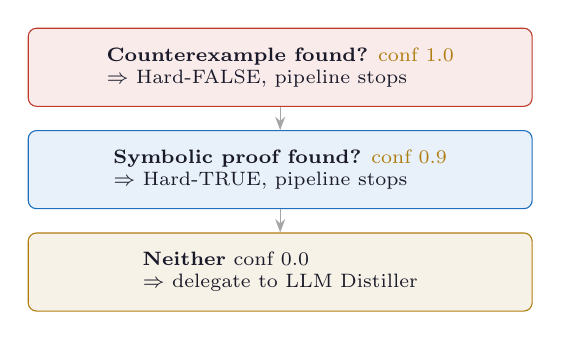
\begin{tikzpicture}[every node/.style={font=\scriptsize},
                        ar/.style={-Stealth,gray!70,thin}]
      \node[draw=AccentRed,   fill=AccentRed!10,   rounded corners=3pt,
            minimum width=6.4cm, inner sep=7pt, align=left, text=TextDark]
        (c1) at (0, 0)
        {\textbf{Counterexample found?}
         \hfill\textcolor{AccentGold}{conf 1.0}\\
         $\Rightarrow$ Hard-FALSE, pipeline stops};
      \node[draw=AccentBlue,  fill=AccentBlue!10,  rounded corners=3pt,
            minimum width=6.4cm, inner sep=7pt, align=left, text=TextDark]
        (c2) at (0,-1.3)
        {\textbf{Symbolic proof found?}
         \hfill\textcolor{AccentGold}{conf 0.9}\\
         $\Rightarrow$ Hard-TRUE, pipeline stops};
      \node[draw=AccentGold,  fill=AccentGold!10,  rounded corners=3pt,
            minimum width=6.4cm, inner sep=7pt, align=left, text=TextDark]
        (c3) at (0,-2.6)
        {\textbf{Neither} \hfill conf 0.0\\
         $\Rightarrow$ delegate to LLM Distiller};
      \draw[ar](c1)--(c2); \draw[ar](c2)--(c3);
    \end{tikzpicture}
    \vspace{2mm}
    \textcolor{gray}{\scriptsize Negative result $\neq$ falsity: the prover is deliberately conservative.}
  \end{column}
\end{columns}
\end{frame}

% ============================================================
% SLIDE 8  ·  LLM DISTILLER
% ============================================================
\begin{frame}{Agent: LLM Distiller}{Qwen2.5-7B + LoRA — Architecture \& inference modes}
\begin{columns}[T,onlytextwidth]
  \begin{column}{0.46\textwidth}
    \vspace{4mm}
    \cy{Model stack:}
    \vspace{5mm}

    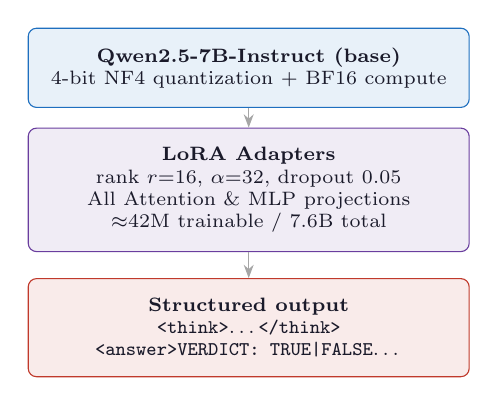
\begin{tikzpicture}[every node/.style={font=\scriptsize},
                        ar/.style={-Stealth,gray!70,thin}]
      \node[draw=AccentBlue,  fill=AccentBlue!10,  rounded corners=3pt,
            minimum width=5.6cm, inner sep=7pt, align=center, text=TextDark]
        (base) at (0,0)
        {\textbf{Qwen2.5-7B-Instruct (base)}\\
         4-bit NF4 quantization + BF16 compute};
      \node[draw=AccentPurple,fill=AccentPurple!10,rounded corners=3pt,
            minimum width=5.6cm, inner sep=7pt, align=center, text=TextDark]
        (lora) at (0,-1.55)
        {\textbf{LoRA Adapters}\\
         rank $r{=}16$,\ $\alpha{=}32$,\ dropout $0.05$\\
         All Attention \& MLP projections\\
         $\approx$42M trainable / 7.6B total};
      \node[draw=AccentRed,   fill=AccentRed!10,   rounded corners=3pt,
            minimum width=5.6cm, inner sep=7pt, align=center, text=TextDark]
        (out) at (0,-3.30)
        {\textbf{Structured output}\\
         \texttt{<think>}\ldots\texttt{</think>}\\
         \texttt{<answer>VERDICT: TRUE|FALSE}\ldots};
      \draw[ar](base)--(lora); \draw[ar](lora)--(out);
    \end{tikzpicture}
  \end{column}
  \hfill
  \begin{column}{0.50\textwidth}
    \vspace{3mm}
    \cy{Two inference modes:}
    \vspace{4mm}

    \begin{block}{Per-problem mode}
      \textbf{Input:} EvidenceBundle + RAG context\\
      \textbf{Output:} chain-of-thought + VERDICT
    \end{block}

    \vspace{3mm}

    \begin{block}{Cheat-sheet synthesis mode}
      \textbf{Input:} cluster of similar problems\\
      \textbf{Output:} $\leq$1\,200-byte lemma block\\
      \texttt{VERDICT} tokens \textbf{banned} in synthesis prompt
    \end{block}

    \vspace{3mm}
    \cy{Why Qwen2.5-7B?}\\[3pt]
    \scriptsize
    Fits in 4-bit on a single GPU $\cdot$
    satisfies the \$0.01/problem budget $\cdot$
    strong mathematical baseline
  \end{column}
\end{columns}
\end{frame}

% ============================================================
% SLIDE 9  ·  DATASET
% ============================================================
\begin{frame}{Dataset}{Training corpus — 4\,694 labelled problems}
\vspace{3mm}

% ── Full-width table ──────────────────────────────────────────
\setlength\arrayrulewidth{0.3pt}
\arrayrulecolor{gray!40}
\begin{tabular}{p{3.8cm}rp{5.4cm}}
  \toprule
  \rowcolor{BannerDark}
  \textcolor{white}{\textbf{Source}} &
  \textcolor{white}{\textbf{\#}} &
  \textcolor{white}{\textbf{Notes}} \\
  \midrule
  \rowcolor{BoxBg}
  SAIR judge repo       & 20           & canonical labelled examples \\
  Playground hard3      & 72           & 40 TRUE / 32 FALSE \\
  \rowcolor{BoxBg}
  Competition dumps     & $\sim$1\,669 & \texttt{hard.txt}, \texttt{hard2.txt}, \texttt{hard3.txt}, \texttt{normales.txt} \\
  Equations (ChromaDB)  & $\sim$2\,933 & embedded RAG index \\
  \midrule
  \rowcolor{BannerDark}
  \textcolor{white}{\textbf{Total}} &
  \textcolor{white}{\textbf{4\,694}} &
  \textcolor{white}{deterministic split, seed 0} \\
  \bottomrule
\end{tabular}

\vspace{5mm}

% ── Two-column: split info  |  image placeholder ─────────────
\begin{columns}[T,onlytextwidth]
  \begin{column}{0.42\textwidth}
    \textbf{Train / Eval split:}\\[4pt]
    \textcolor{AccentBlue}{\textbf{80\%}} train — 3\,755 problems\\[2pt]
    \textcolor{AccentRed}{\textbf{20\%}} eval \phantom{0}— 939 problems

    \vspace{5mm}
    \textcolor{gray}{\scriptsize
      Problems where pipeline verdict $\neq$ ground truth
      are excluded from SFT.\\
      $\sim$1\,330 clean examples used.}
  \end{column}
  \hfill
  \begin{column}{0.54\textwidth}
    % IMAGE PLACEHOLDER
    % Suggested: two subplots (matplotlib, light bg).
    % Left: pie/bar of data source breakdown (4 slices).
    % Right: stacked bar TRUE/FALSE per difficulty level
    %        (normal / hard / hard2 / hard3).
    % Colors: AccentBlue / AccentGreen / AccentGold / AccentRed.
    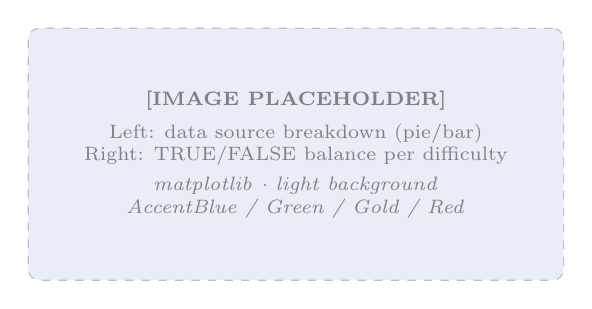
\begin{tikzpicture}
      \node[draw=gray!50, dashed, fill=BoxBg, rounded corners=4pt,
            minimum width=6.8cm, minimum height=3.2cm,
            align=center, text=gray, font=\scriptsize]{%
        \textbf{[IMAGE PLACEHOLDER]}\\[4pt]
        Left: data source breakdown (pie/bar)\\
        Right: TRUE/FALSE balance per difficulty\\[3pt]
        \textit{matplotlib · light background}\\
        \textit{AccentBlue / Green / Gold / Red}
      };
    \end{tikzpicture}
  \end{column}
\end{columns}
\end{frame}

% ============================================================
% SLIDE 10  ·  SFT
% ============================================================
\begin{frame}{Training Stage 1}{Supervised Fine-Tuning (SFT)}
\begin{columns}[T,onlytextwidth]
  \begin{column}{0.50\textwidth}
    \vspace{4mm}
    \cy{EvidenceBundle $\to$ structured completion:}
    \vspace{4mm}

    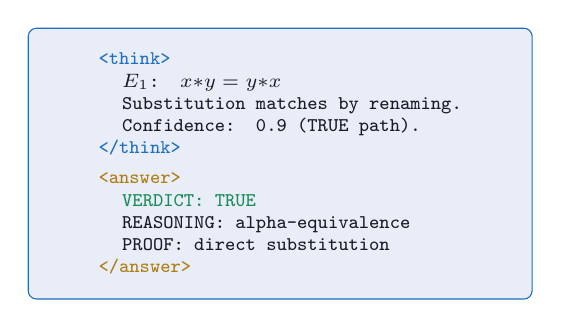
\begin{tikzpicture}
      \node[draw=AccentBlue, fill=BoxBg, rounded corners=3pt,
            minimum width=6.4cm, inner sep=9pt,
            align=left, text=TextDark, font=\ttfamily\scriptsize]{%
        \textcolor{AccentBlue}{<think>}\\
        \hspace{3mm}$E_1$: $x{*}y = y{*}x$\\
        \hspace{3mm}Substitution matches by renaming.\\
        \hspace{3mm}Confidence: 0.9 (TRUE path).\\
        \textcolor{AccentBlue}{</think>}\\[3pt]
        \textcolor{AccentGold}{<answer>}\\
        \hspace{3mm}\textcolor{AccentGreen}{VERDICT: TRUE}\\
        \hspace{3mm}REASONING: alpha-equivalence\\
        \hspace{3mm}PROOF: direct substitution\\
        \textcolor{AccentGold}{</answer>}
      };
    \end{tikzpicture}
  \end{column}
  \hfill
  \begin{column}{0.46\textwidth}
    \vspace{4mm}
    \cy{Hyperparameters:}
    \vspace{4mm}

    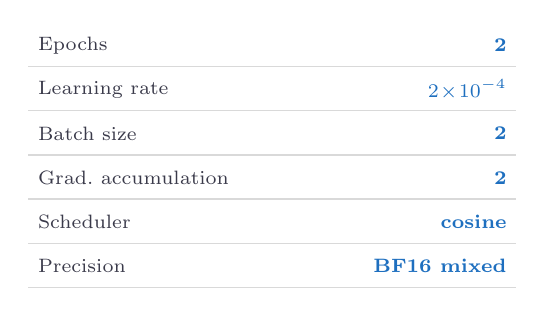
\begin{tikzpicture}[every node/.style={font=\scriptsize}]
      \foreach \k/\v/\i in {
        Epochs/2/0,
        {Learning rate}/$2\!\times\!10^{-4}$/1,
        {Batch size}/2/2,
        {Grad.\ accumulation}/2/3,
        Scheduler/cosine/4,
        Precision/{BF16 mixed}/5%
      }{
        \pgfmathsetmacro\yy{-\i * 0.56}
        \node[anchor=west, text=TextMid] at (0,\yy) {\k};
        \node[anchor=east, text=AccentBlue, font=\scriptsize\bfseries]
          at (6.2,\yy) {\v};
        \draw[gray!30, thin] (0,\yy-0.27) -- (6.2,\yy-0.27);
      }
    \end{tikzpicture}

    \vspace{6mm}
    \begin{block}{Goal}
      Teach the model \textit{format compliance} first.
      GRPO will then optimise verdict correctness.
    \end{block}
  \end{column}
\end{columns}
\end{frame}

% ============================================================
% SLIDE 11  ·  GRPO
% ============================================================
\begin{frame}{Training Stage 2}{GRPO — Reinforcement Learning from Verifier Feedback}
\begin{columns}[T,onlytextwidth]
  \begin{column}{0.52\textwidth}
    \vspace{4mm}
    \cy{Reward function:}
    \vspace{3mm}

    {\scriptsize
    \begin{align*}
      R \;=\; &\underbrace{0.70\cdot\mathbf{1}[\text{verdict correct}]}_{\text{dominant}}
               + 0.10\cdot\mathbf{1}[\texttt{<answer>}]\\
              &+ 0.10\cdot\mathbf{1}[\text{struct.}]
               + 0.05\cdot\mathbf{1}[\texttt{<think>}]
               + 0.05\cdot\mathbf{1}[\text{fallback}]
    \end{align*}
    }

    \vspace{4mm}
    % Reward breakdown bars
    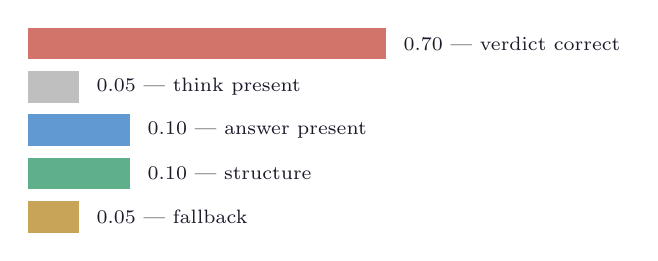
\begin{tikzpicture}[every node/.style={font=\scriptsize}]
      \fill[AccentRed!70]   (0,0.00) rectangle (4.55,0.40);
      \node[anchor=west, text=TextDark] at (4.65,0.20) {0.70 — verdict correct};
      \fill[gray!50]        (0,-0.55) rectangle (0.65,-0.15);
      \node[anchor=west, text=TextDark] at (0.75,-0.35) {0.05 — think present};
      \fill[AccentBlue!70]  (0,-1.10) rectangle (1.30,-0.70);
      \node[anchor=west, text=TextDark] at (1.40,-0.90) {0.10 — answer present};
      \fill[AccentGreen!70] (0,-1.65) rectangle (1.30,-1.25);
      \node[anchor=west, text=TextDark] at (1.40,-1.45) {0.10 — structure};
      \fill[AccentGold!70]  (0,-2.20) rectangle (0.65,-1.80);
      \node[anchor=west, text=TextDark] at (0.75,-2.00) {0.05 — fallback};
    \end{tikzpicture}
  \end{column}
  \hfill
  \begin{column}{0.44\textwidth}
    \vspace{4mm}
    \cy{GRPO algorithm:}
    \vspace{5mm}

    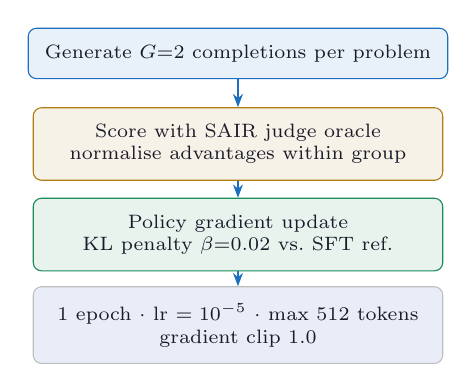
\begin{tikzpicture}[every node/.style={font=\scriptsize},
                        ar/.style={-Stealth,thin,AccentBlue}]
      \node[draw=AccentBlue, fill=AccentBlue!10, rounded corners=3pt,
            minimum width=5.2cm, inner sep=6pt, align=center, text=TextDark]
        (g1) at (0,0) {Generate $G{=}2$ completions per problem};
      \node[draw=AccentGold, fill=AccentGold!10, rounded corners=3pt,
            minimum width=5.2cm, inner sep=6pt, align=center, text=TextDark]
        (g2) at (0,-1.15)
        {Score with SAIR judge oracle\\normalise advantages within group};
      \node[draw=AccentGreen,fill=AccentGreen!10,rounded corners=3pt,
            minimum width=5.2cm, inner sep=6pt, align=center, text=TextDark]
        (g3) at (0,-2.30)
        {Policy gradient update\\KL penalty $\beta{=}0.02$ vs.\ SFT ref.};
      \node[draw=gray!50, fill=BoxBg, rounded corners=3pt,
            minimum width=5.2cm, inner sep=6pt, align=center, text=TextDark]
        (g4) at (0,-3.45)
        {1 epoch $\cdot$ lr $= 10^{-5}$ $\cdot$ max 512 tokens\\gradient clip 1.0};
      \draw[ar](g1)--(g2); \draw[ar](g2)--(g3); \draw[ar](g3)--(g4);
    \end{tikzpicture}
  \end{column}
\end{columns}
\end{frame}

% ============================================================
% SLIDE 12  ·  CHEAT SHEET DISTILLATION
% ============================================================
\begin{frame}{Cheat Sheet Distillation}{Stage 3 — Offline knowledge compression}
\begin{columns}[T,onlytextwidth]
  \begin{column}{0.46\textwidth}
    \vspace{4mm}
    \cy{Pipeline:}
    \vspace{5mm}

    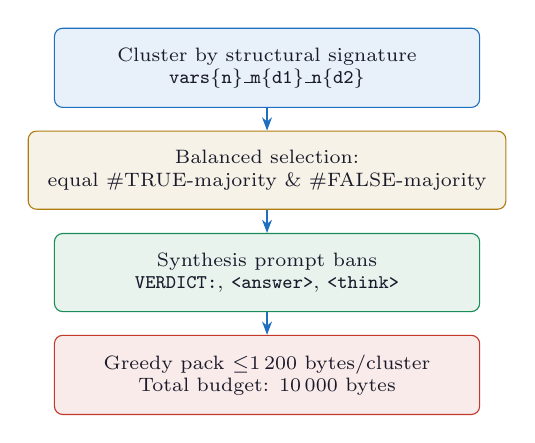
\begin{tikzpicture}[every node/.style={font=\scriptsize},
                        ar/.style={-Stealth,thin,AccentBlue}]
      \node[draw=AccentBlue, fill=AccentBlue!10, rounded corners=3pt,
            minimum width=5.4cm, inner sep=7pt, align=center, text=TextDark]
        (s1) at (0,0)
        {Cluster by structural signature\\
         \texttt{vars\{n\}\_m\{d1\}\_n\{d2\}}};
      \node[draw=AccentGold, fill=AccentGold!10, rounded corners=3pt,
            minimum width=5.4cm, inner sep=7pt, align=center, text=TextDark]
        (s2) at (0,-1.3)
        {Balanced selection:\\
         equal \#TRUE-majority \& \#FALSE-majority};
      \node[draw=AccentGreen,fill=AccentGreen!10,rounded corners=3pt,
            minimum width=5.4cm, inner sep=7pt, align=center, text=TextDark]
        (s3) at (0,-2.6)
        {Synthesis prompt bans\\
         \texttt{VERDICT:}, \texttt{<answer>}, \texttt{<think>}};
      \node[draw=AccentRed,  fill=AccentRed!10,  rounded corners=3pt,
            minimum width=5.4cm, inner sep=7pt, align=center, text=TextDark]
        (s4) at (0,-3.9)
        {Greedy pack $\leq$1\,200 bytes/cluster\\
         Total budget: 10\,000 bytes};
      \draw[ar](s1)--(s2); \draw[ar](s2)--(s3); \draw[ar](s3)--(s4);
    \end{tikzpicture}
  \end{column}
  \hfill

  \begin{column}{0.50\textwidth}
    \vspace{3mm}
    \cy{v1 failure \& v2 fix:}
    \vspace{4mm}

    \begin{alertblock}{v1 — Collapsed to 20\% accuracy}
      FALSE-dominated clusters leaked verdict tokens
      into synthesis $\Rightarrow$ systematic bias toward FALSE
    \end{alertblock}

    \vspace{4mm}

    \begin{exampleblock}{v2 — Balanced clustering}
      Enforce equal TRUE/FALSE cluster counts +
      dedicated synthesis prompt forbids verdict tokens
    \end{exampleblock}

    \vspace{4mm}
    \cy{Preamble entry (priority 999):}
    \vspace{2mm}

    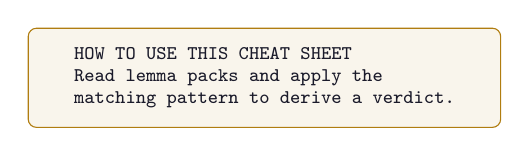
\begin{tikzpicture}
      \node[draw=AccentGold, fill=AccentGold!8, rounded corners=3pt,
            minimum width=6.0cm, inner sep=7pt,
            align=left, text=TextDark, font=\ttfamily\scriptsize]{%
        HOW TO USE THIS CHEAT SHEET\\
        Read lemma packs and apply the\\
        matching pattern to derive a verdict.
      };
    \end{tikzpicture}
  \end{column}
\end{columns}
\end{frame}

% ============================================================
% SLIDE 13  ·  DISTILL THEN DEPLOY
% ============================================================
\begin{frame}{Distill, Then Deploy}{Offline training vs.\ online evaluation}
\vspace{4mm}
\centering
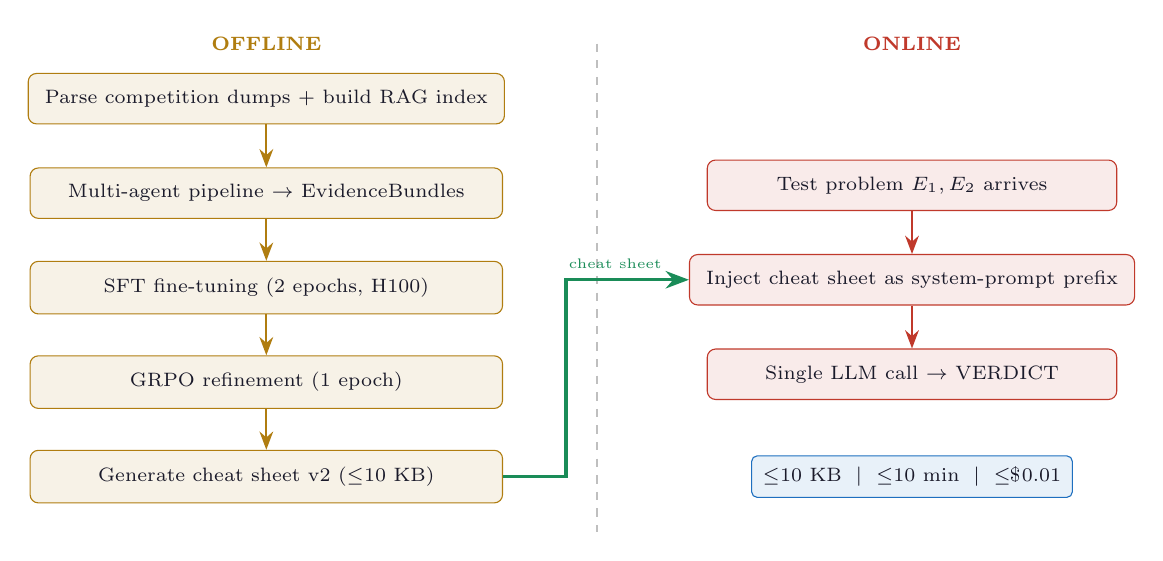
\begin{tikzpicture}[
  every node/.style={font=\scriptsize},
  OF/.style={draw=AccentGold,  fill=AccentGold!10,  rounded corners=3pt,
             minimum width=6.0cm, inner sep=6pt, align=center, text=TextDark},
  ON/.style={draw=AccentRed,   fill=AccentRed!10,   rounded corners=3pt,
             minimum width=5.2cm, inner sep=6pt, align=center, text=TextDark},
  ar/.style={-Stealth, thick},
]
  % OFFLINE
  \node[OF] (o1) at (-4.2, 2.0) {Parse competition dumps + build RAG index};
  \node[OF] (o2) at (-4.2, 0.8) {Multi-agent pipeline $\to$ EvidenceBundles};
  \node[OF] (o3) at (-4.2,-0.4) {SFT fine-tuning (2 epochs, H100)};
  \node[OF] (o4) at (-4.2,-1.6) {GRPO refinement (1 epoch)};
  \node[OF] (o5) at (-4.2,-2.8) {Generate cheat sheet v2 ($\leq$10 KB)};
  \foreach \a/\b in {o1/o2,o2/o3,o3/o4,o4/o5}
    \draw[ar,AccentGold](\a)--(\b);

  % ONLINE
  \node[ON] (e1) at (4.0, 0.9) {Test problem $E_1, E_2$ arrives};
  \node[ON] (e2) at (4.0,-0.3) {Inject cheat sheet as system-prompt prefix};
  \node[ON] (e3) at (4.0,-1.5) {Single LLM call $\to$ VERDICT};
  \foreach \a/\b in {e1/e2,e2/e3}
    \draw[ar,AccentRed](\a)--(\b);

  % Divider
  \draw[dashed,gray!50,thick](0,2.7)--(0,-3.5);
  \node[font=\scriptsize\bfseries, text=AccentGold] at (-4.2, 2.7) {OFFLINE};
  \node[font=\scriptsize\bfseries, text=AccentRed]  at ( 4.0, 2.7) {ONLINE};

  % Bridge
  \draw[ar,AccentGreen,very thick]
    (o5.east) -- ++(8mm,0) |- ([yshift=0mm]e2.west)
    % node[pos=0.42, above, font=\tiny, text=AccentGreen]{cheat sheet};
    node[pos=0.70, above, font=\tiny, text=AccentGreen]{cheat sheet};

  % Constraint badge
  \node[draw=AccentBlue, fill=AccentBlue!10, rounded corners=2pt,
        font=\scriptsize, text=TextDark, inner sep=4pt] at (4.0,-2.8)
    {$\leq$10 KB $\;|\;$ $\leq$10 min $\;|\;$ $\leq$\$0.01};
\end{tikzpicture}
\end{frame}

% ============================================================
% SLIDE 14  ·  RESULTS
% ============================================================
\begin{frame}{Experimental Results}{Accuracy across training configurations}
\begin{columns}[T,onlytextwidth]
  \begin{column}{0.46\textwidth}
    \vspace{4mm}
    \cy{Performance table:}
    \vspace{3mm}

    \setlength\arrayrulewidth{0.3pt}
    \arrayrulecolor{gray!40}
    \begin{tabular*}{\linewidth}{@{\extracolsep{\fill}}lcc}
      \toprule
      \rowcolor{BannerDark}
      \textcolor{white}{\textbf{Configuration}} &
      \textcolor{white}{\textbf{Acc.}} &
      \textcolor{white}{\textbf{Parse}} \\
      \midrule
      \rowcolor{BoxBg}
      Base model (no fine-tuning)    & 0.50 & 0.75 \\
      Symbolic agents only           & 0.50 & ---  \\
      \rowcolor{BoxBg}
      SFT only (20-problem corpus)   & 0.75 & 1.00 \\
      SFT + GRPO (20-problem corpus) & 0.75 & 1.00 \\
      \rowcolor{AccentRed!15}
      + cheat sheet \textbf{v1}
        & \textcolor{AccentRed}{\textbf{0.20}} & 1.00 \\
      \rowcolor{AccentGreen!15}
      + cheat sheet \textbf{v2}
        & \textcolor{AccentGreen}{\textbf{in prog.}} & 1.00 \\
      \bottomrule
    \end{tabular*}

    \vspace{5mm}
    \textcolor{gray}{\scriptsize
      Training infrastructure: DGX cluster ($8\times$ NVIDIA H100)}
  \end{column}
  \hspace{0.03\textwidth}
  \begin{column}{0.46\textwidth}
    \vspace{4mm}
    % IMAGE PLACEHOLDER
    % Suggested: matplotlib bar chart (light background).
    % X-axis: Base / SFT / SFT+GRPO / v1 / v2
    % Y-axis: accuracy 0.0–1.0
    % Annotate v1 bar in AccentRed with label "FALSE bias".
    % v2 bar in AccentGreen marked "in progress".
    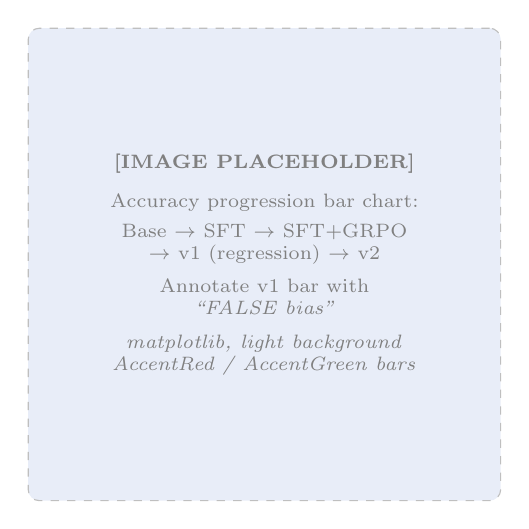
\begin{tikzpicture}
      \node[draw=gray!50, dashed, fill=BoxBg,
            rounded corners=4pt, minimum width=6.0cm, minimum height=6.0cm,
            align=center, text=gray, font=\scriptsize]{%
        \textbf{[IMAGE PLACEHOLDER]}\\[6pt]
        Accuracy progression bar chart:\\[3pt]
        Base $\to$ SFT $\to$ SFT+GRPO\\
        $\to$ v1 (regression) $\to$ v2\\[4pt]
        Annotate v1 bar with\\
        \textit{``FALSE bias''}\\[4pt]
        \textit{matplotlib, light background}\\
        \textit{AccentRed / AccentGreen bars}
      };
    \end{tikzpicture}
  \end{column}
\end{columns}
\end{frame}

% ============================================================
% SLIDE 15  ·  CONCLUSIONS
% ============================================================
{
\setbeamertemplate{footline}{}
\begin{frame}[plain]
\begin{tikzpicture}[remember picture,overlay]
  \fill[BannerDark] (current page.north west)
    rectangle ([yshift=-22mm]current page.north east);
  \node[font=\large\bfseries, text=white,
        anchor=north west, xshift=8mm, yshift=-5mm]
    at (current page.north west) {Conclusions \& Future Work};
  \node[font=\scriptsize, text=AccentCyan,
        anchor=north west, xshift=8mm, yshift=-15mm]
    at (current page.north west) {ARD — Algebraic Reasoning Distiller};
  % footer bar
  \fill[BannerMid] (current page.south west)
    rectangle ([yshift=6mm]current page.south east);
  \node[font=\tiny, text=gray,
        anchor=south, yshift=1.5mm] at (current page.south)
    {Joaquín Mir Macías $\cdot$ José Andrés Ridruejo Tuñón $\cdot$
     Javier Ríos Montes $\cdot$ Miguel Montes Lorenzo $\cdot$
     Deep Generative Models $\cdot$ UPM 2025/2026};
\end{tikzpicture}

\vspace{20mm}
\begin{columns}[T,onlytextwidth]
  \begin{column}{0.50\textwidth}
    \cy{Key contributions:}
    \vspace{2mm}
    \begin{itemize}\setlength\itemsep{3pt}
      \item[\textcolor{AccentGreen}{$\checkmark$}]
        Multi-agent pipeline: \textbf{symbolic} + \textbf{neural} reasoning
      \item[\textcolor{AccentGreen}{$\checkmark$}]
        SFT $\to$ GRPO within \textbf{severe resource constraints}
      \item[\textcolor{AccentGreen}{$\checkmark$}]
        Identified \& fixed cheat-sheet \textbf{verdict-bias} (v1 $\to$ v2)
      \item[\textcolor{AccentGreen}{$\checkmark$}]
        Reproducible on DGX (Docker + \texttt{uv})
    \end{itemize}
    \vspace{3mm}
    \cy{Lessons learned:}\\[2pt]
    \scriptsize Data \textbf{balance} is critical. Synthesis prompt must
    \textit{decouple} generation from judgment.
    Graceful degradation enables robust deployment.
  \end{column}
  \hfill
  \begin{column}{0.46\textwidth}
    \gd{Future work:}
    \vspace{2mm}
    \begin{itemize}\setlength\itemsep{3pt}
      \item[\textcolor{AccentGold}{$\triangleright$}]
        Complete cheat sheet \textbf{v2} on full 1\,761-problem corpus
      \item[\textcolor{AccentGold}{$\triangleright$}]
        Order-4 \textbf{exhaustive} magma search
      \item[\textcolor{AccentGold}{$\triangleright$}]
        Distil into \textbf{smaller models} ($<$3B params)
      \item[\textcolor{AccentGold}{$\triangleright$}]
        Iterative cheat-sheet refinement via GRPO loop
    \end{itemize}
    \vspace{3mm}
    % \begin{tikzpicture}
    %   \node[draw=AccentBlue, fill=AccentBlue!10, rounded corners=4pt,
    %         % inner sep=7pt, align=center, text=TextDark, font=\scriptsize]{%
    %         inner sep=7pt, align=center, text=TextDark, font=\scriptsize]{%
    %     \textbf{Repository:} MIT Licensed\\
    %     github.com/joaquinmaciias/Algebraic-Reasoning-Distiller.git
    %   };
    % \end{tikzpicture}
    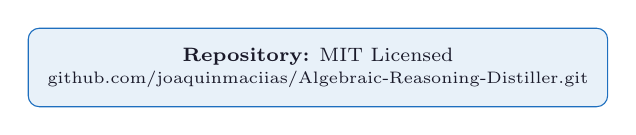
\begin{tikzpicture}
      \node[draw=AccentBlue, fill=AccentBlue!10, rounded corners=4pt,
            inner sep=7pt, align=center, text=TextDark, font=\scriptsize]{%
        \textbf{Repository:} MIT Licensed\\
        {\fontsize{6.5pt}{7.5pt}\selectfont
        github.com/joaquinmaciias/Algebraic-Reasoning-Distiller.git}
      };
    \end{tikzpicture}
  \end{column}
\end{columns}
\end{frame}
}

\end{document}